\documentclass[11pt]{report}

\usepackage[utf8]{inputenc}
\usepackage[T1]{fontenc}
\usepackage{geometry}
\geometry{hmargin=3cm,vmargin=2.5cm}
%\usepackage[top=2cm, bottom=2cm, left=2cm, right=2cm]{geometry}
\usepackage{color}
\usepackage{setspace}
\usepackage{listings}
\lstdefinelanguage{AnnJava}[]{Java}%
    {morekeywords={@DefineGroups,@DefineRules,@Compatible,@Group,@MemberOf}}
\usepackage{graphicx}
\usepackage{algorithm}
\usepackage{cite}
\newcommand{\TODO}[1]{\textcolor{red}{\textbf{[TODO:#1]}}}

\begin{document}
% Interligne à 1.5
\onehalfspacing
% ajout du titre
\begin{titlepage}

\newcommand{\HRule}{\rule{\linewidth}{0.5mm}} % Defines a new command for the horizontal lines, change thickness here

\center % Center everything on the page
 
%----------------------------------------------------------------------------------------
%	HEADING SECTIONS
%----------------------------------------------------------------------------------------
\textbf{}\\[0.5cm]
\textsc{\LARGE University of Nice Sophia Antipolis}\\[1cm] % Name of your university/college
\textsc{\Large Master IFI - Ubinet track}\\[0.5cm] % Major heading such as course name
\textsc{\large master thesis}\\[0.5cm] % Minor heading such as course title

%----------------------------------------------------------------------------------------
%	TITLE SECTION
%----------------------------------------------------------------------------------------

\HRule \\[0.4cm]
{ \huge \bfseries Request Scheduling for multiactive objects}\\[0.4cm] % Title of your document
\HRule \\[1cm]
 
%----------------------------------------------------------------------------------------
%	AUTHOR SECTION
%----------------------------------------------------------------------------------------
\begin{minipage}{0.48\textwidth}
\center
\Large \emph{Student}\\
Justine \textsc{Rochas}\\[0.5cm]% Your name
\emph{Internship Supervisor} \\
Ludovic \textsc{Henrio}\\[0.5cm]% Supervisor's Name
\emph{Academic Supervisor} \\
Dino \textsc{Lopez}\\[0.5cm]% Supervisor's Name
\end{minipage}
~
\begin{minipage}{0.48\textwidth}
\center
\Large \emph{Research Lab}\\
\textsc{INRIA-I3S-CNRS-UNS} \\[0.5cm]% Your name
\emph{Research Project-Team}\\
\textsc{OASIS}\\[0.5cm] % Your name
\end{minipage}\\[4cm]

\begin{figure}[!t]

\includegraphics[width=4cm]{pictures/logo.jpg} 
\end{figure}


% If you don't want a supervisor, uncomment the two lines below and remove the section above
%\Large \emph{Author:}\\
%John \textsc{Smith}\\[3cm] % Your name

%----------------------------------------------------------------------------------------
%	DATE SECTION
%----------------------------------------------------------------------------------------

{\large August 30, 2013}\\[3cm] % Date, change the \today to a set date if you want to be precise

%----------------------------------------------------------------------------------------
%	LOGO SECTION
%----------------------------------------------------------------------------------------

%\includegraphics{Logo}\\[1cm] % Include a department/university logo - this will require the graphicx package

 
%----------------------------------------------------------------------------------------

\vfill % Fill the rest of the page with whitespace

\end{titlepage}

 
\begin{abstract}
The active object programming model aims to facilitate the writing of distributed applications. It provides asynchronous remote method calls and mechanisms to prevent data races. However this model does not take advantage of multicore architectures as it is intrinsically mono-threaded. To overcome this problem, a recent extension of the active object model has been designed, which is called the multiactive object model. Multiactive objects enable local parallelism at a high level without giving up simplicity and safety provided by active objects: the programmer can declare which requests can be run in parallel through a customized specification language. However, in this new model, the programmer has not yet control on the scheduling policy applied on the requests executed by a multiactive object. In this work, we study application-level scheduling concepts that can be applied to multiactive objects. The goal is to allow the programmer to have a fine control on the scheduling policy through simple specifications. We first develop a priority mechanism that can be used to reorder awaiting requests in the queue of multiactive objects. Second, we provide a simple thread management mechanism to better allocate available threads to awaiting requests. Finally, we experiment the new features in a practical context, showing that the proposed mechanisms increase the efficiency of multiactive objects while keeping a low overhead. On the whole, we provide general specifications for application-level scheduling that are together fine-grained, user-friendly, and efficient.

\end{abstract}

\tableofcontents
\newpage

\chapter{Introduction}
\section{Motivation}
%\section{Context, Motivation, General Objectives}
Writing distributed applications is tremendous. There are a lot of aspects in distributed programming that differ from local programming: naming, localization, timing, network reliance, etc. In order to ease distributed programming, specialized APIs, middlewares and distributed models are being developed. They attempt to hide remoteness the best they can by relying on generated code and fault tolerant protocols. Designing such protocols requires a deep understanding of language semantics. The object-oriented paradigm has been shown to be well adapted to abstract distribution, because (i) by definition, an object is something that can stand alone, which makes it easy to distribute, and because (ii) inheritance can be used to specialized a local method call into a remote method call. The RMI Java API \cite{ref:rmi} is a successful example of distribution abstraction; it provides classes that must be used to make remote objects communicate. 

In the same idea, the Active Object model \cite{ref:Lavender95activeobject} is an example of programming model that is meant for distribution and that is suited to any object-oriented languages. In this model, objects are seen as independent entities that execute in their own thread. Active objects communicate with each other via asynchronous method calls, unlike RMI (which supports only synchronous communications). The semantics of a method invocation is thus different whether it is remote or local.
In the particular implementation of active objects we study in this work, the same syntax is applied whether a method call is remote or local. Most of the distribution aspects are integrated when creating an active object: communication details are dealt separately from the business code. This completely hides distribution, which makes distributed code easier to write. 

More recently, the same kind of abstraction emerged for concurrent programming. The goal is to give opportunity to the programmer to fully use the parallelism of computing units, without having to be an expert in concurrent programming. Again, static and dynamic analysis can be automatically made such that the parallelism is directly extracted from the code, or simply declared by the programmer via a high level declaration language. For example, some C and C++ \emph{pragmas} (preprocessor directives) \cite{ref:openmp} are devoted to parallelism and allow the programmer to indicate that some part of code should be parallelized at runtime according to several parameters. Here again, concurrency matters are isolated from business code, and producing parallel code is made easier.

\paragraph{}
In this objective, the OASIS research team has developed a new model built on top of the active object model, that gathers both distribution and concurrency abstractions. This new model is called the Multiactive Object model. It keeps the same convenience for distribution as active objects. In addition, this model provides facilities for the programmer to be able to define safe parallel executions within an active object. In this model, parallelism applies on requests (a multiactive object can execute several requests at the same time). Parallelism applies then on a higher level than \emph{pragmas}, which usually apply to small parts of code. The concurrency model offered by multiactive objects is more convenient than existing low level concurrency mechanisms, such as locks and semaphores \cite{ref:semaphore},
because those tools are very permissive and error prone, whereas multiactive objects automatically block execution of requests that do not satisfy the programmer's specification.
Thus, multiactive objects avoid data races that could be due to a lack of concurrency knowledge from the programmer.

The multiactive object model provides request-level parallelism thanks to the specifications written by the programmer.
Currently, to execute requests, multiactive objects enforce an adapted FIFO policy for parallel safe execution. As multiactive objects rely on a limited number of threads to execute requests, it is possible that some requests wait in the queue even if they are ready to execute safely.
As a consequence, it would be convenient to be able to reorder requests that are waiting in the queue according to their importance. But the programmer cannot assign yet priority of execution in multiactive objects, which should be a crucial functionality in a concurrent context. The programmer cannot influence either the way the threads are allocated: if a ready-to-execute request is first in the queue, then it is allocated the next available thread, regardless of how many identical request already execute. In brief, the scheduling policy applied in a multiactive object is not controllable from the programmer perspective. In this work, we attempt to empower the programmer with the ability to impact on the request scheduling of multiactive objects. The contributions of this work are  threefold. 

\begin{itemize}
\item First, we  provide a new specification language to indicate priority of requests, we show that is easy to use and expressive.
\item Second, we provide a mechanism to partition the available threads among the requests. Through this mechanism, we aim to avoid starvation of requests.
\item Third, we experiment those mechanisms in various ways, showing that they successfully increase the throughput of most important requests and that they do not introduce a worrying overhead.
\end{itemize}

In summary, we provide efficient tools that allow the programmer to have more control on the scheduling policy of multiactive objects. As a consequence, those tools increase efficiency of multiactive objects.


\section{Organization of the report}
The report is organized as follows. Chapter 2 introduces the background, which is, on one hand, active objects and their main existing implementations, and on the other hand, multiactive objects and its current implementation. Then the detailed objectives of the internship are presented considering the background. Finally, Chapter 2 exposes related works on high-level scheduling, either in the context of active objects or of meta programming.

Chapter 3 describes the contributions in detail. In particular, it introduces the two priority specifications that have been developed and states their main properties. It also exposes the thread allocation problem that arises from the introduction of priorities, and the solutions that have been given to this problem. Then, Chapter 3 exposes experimental evaluations showing that the priorities significantly speed up the processing of high priority requests. We also show that our priority specification keeps a low overhead even if  it is a very high level specification language.

Finally, Chapter 4 concludes and gives an outline for future works.

\chapter{Background and Related Works}
\section{Active Objects}
In this section, we first present in details the principles of the particular implementation of active objects that is the basis of our work, and then we review other existing active object implementations and compare them with our definition.

\subsection{Principles}\label{sec:activeobjects}
The active object model is a programming model that facilitates the writing of distributed applications. This model is not tight to a particular programming language. It can be applied to any object-oriented language. In this model, certain objects can be marked as "active", so that their methods can be invoked from remote machines, accessible through the network. The code related to the network calls is thus generated and does not appear in the business code. But active objects provide more than remote method call facilities, which is what differentiates them from lower level remote call mechanisms such as RPC (Remote Procedure Call)\cite{ref:rpc} or in an object-oriented context, RMI (Remote Method Invocation)\cite{ref:rmi}. Indeed, active objects have other properties that ensure both loose coupling of remote entities and safety of execution. More precisely, the three main characteristics of active objects are:
\begin{itemize}
\item Asynchronous remote method calls
\item Absence of local concurrency of requests
\item Absence of shared memory between active objects
\end{itemize}

Those characteristics differ from one implementation of active objects to another. We present below the particular implementation of active objects which is the basis of our work, that is called ASP~\cite{ref:asp}.

\paragraph{}
The first characteristic of active objects is that they provide asynchronous remote calls: the remote calls are not blocking from the program that performs them. It means that the calling program might continue its execution before receiving the result of the call, if the result is not needed right away. Instead of the actual result, a promise of response is given to the caller. This promise of response is known as a \emph{future} \cite{ref:Halstead:1985:MLC:4472.4478}. A future is an object that is a placeholder for the return value of the call. It is created transparently and behaves like the return value (i.e. it inherits from the return value). A future contains code to handle the case in which the result is accessed after the call but before the reception of the result. This is how asynchronous calls are made possible.
The resynchronization occurs then implicitly when accessing the future. There are two kinds of accesses when reading a future. The first kind of access is called a non strict operation, and lets the future behave in place of the result. For example, a non strict operation is an affectation, or a parameter of method call, where the value of the object is not truly needed, only its reference is needed. The second kind of access is called strict operation, and require the future to block the execution until the result is received, if it is not received already. This is where the resynchronization takes place if needed. For example, a strict operation is an increment or a method call on the result, when the actual value of the result is needed.
Figure~\ref{fig:strict_operation} is an example of asynchronous call when using active objects.

\begin{figure}[!ht]
	\lstset{language=java, numbers=left, numberstyle=\tiny, stepnumber=1, numbersep=5pt, basicstyle=\footnotesize}
	\begin{lstlisting}[frame=single]
// Suppose that actObj is an active object
Result res = actObj.produceResult();  // This triggers an asynchronous call

// Both following instructions do not block even if res is not received from 
// actObj when executing those instructions
Result resSaver = res;
resUser.foo(res);

// This instruction blocks until the value of res is received 
// It is a strict operation
res.bar();
 	\end{lstlisting}
\caption{Code illustrating strict and non strict operation on a future}
\label{fig:strict_operation}
\end{figure}

At line 2, a remote call is transparently performed on \textbf{actObj}. The line 6 is executed just after line 2 (in fact, just after the method call is received by \textbf{actObj}), without waiting for the \textbf{res} variable to be fulfilled. Instead, a future object inheriting of the Result class is put in the \textbf{res} variable. Likewise, line 7 is executed without blocking, the future object is actually given as parameter of the method call. In all cases, the execution is continued up to line 11 even if the true value of \textbf{res} is not received up to this point. Line 11 is an implicit synchronization barrier because the actual value of \textbf{res} is needed to perform the \textbf{bar} method on it. The execution here blocks until the value of \textbf{res} is received. In this case, it is the future itself that is in charge of blocking the execution; indeed, the future contains code to handle this case. This behavior is called \emph{wait-by-necessity}, because the execution only blocks when truly needed. 
Note that the behavior of the program is still predictable when using futures because it has a semantics close to a sequential execution, thanks to the wait-by-necessity property and thanks to the language design itself. 

In the following we will talk more generally about \emph{requests} instead of method calls, because this terminology better fit to the asynchronous characteristic.

\paragraph{}
The second characteristic of active objects is the absence of local concurrency. Indeed, the active object model ensures that requests that are sent to an active object are executed sequentially, even if several requests are received "at the same time"; at each moment, a single request is active.
This is possible because an active object embeds a request queue (see Figure~\ref{fig:active_object}).
\begin{figure}[ht]
      \fbox{
      \begin{minipage}[c]{\textwidth}
      \centering
      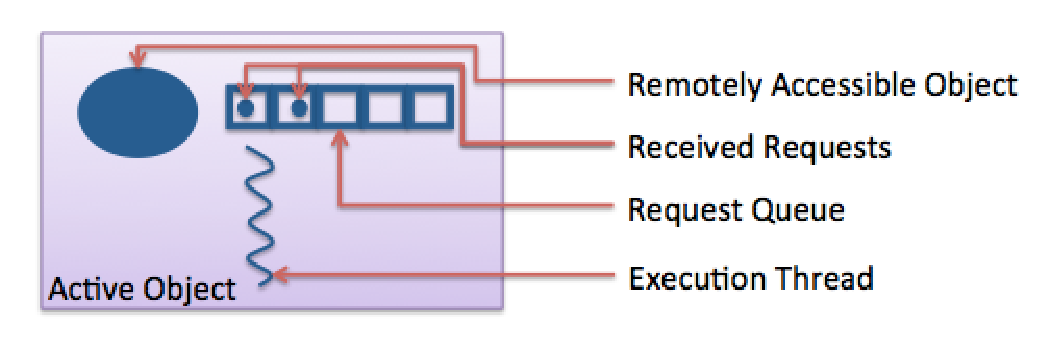
\includegraphics[scale=0.5]{pictures/active_object.pdf}
      \end{minipage}
      }
      \caption{Anatomy of an active object}
      \label{fig:active_object}
\end{figure}
Whenever a request is sent to the active object, this request is automatically put in the queue. Then, the execution thread of an active object executes requests that are in its queue, one at a time. In the particular implementation we describe, when a request body is started, it must be finished before beginning another request body. There is absolutely no overlapping of request executions within an active object.
This simple rule ensures that no data race can exist within an active object. A data race is a concurrent access to a shared resource that can lead to inconsistent state of the resource. For example, if two operations that assign a value to the same variable occur concurrently, then the result is unpredictable since it depends on the interleaving of the operations.
Such situations cannot arise in mono-threaded environments. This is why active objects force a complete sequential execution of requests, so that no data race can then exist.

\paragraph{}
In summary, when using active objects to write distributed applications, the programmer does not need (i) to write the code that performs the remote call and that waits for the reply (because this is handled transparently by the active object), (ii) neither to take care of concurrency problems that can arise when several requests are received at the same time. Both mechanisms facilitate the writing of distributed code and ensure that a correct output is always produced.

From now we are going to focus on the second characteristic of active objects, that is absence of local concurrency. We are going to see in Section~\ref{sec:MAOprinciples} how this strict model is partially released to reintroduce local concurrency without loosing safety of execution. The goal is clearly to gain in efficiency.

\subsection{An overview of active object languages}
In this section, we review existing programming languages that use the active object model. They have slight differences in their implementation of active objects, firstly in the way the asynchronous calls are handled, and secondly in the way the absence of local concurrency is handled. Here we will mainly focus on the second point as it is the most relevant in the context of designing scheduling policies.

\subsubsection{Creol}\label{sec:Creol}
In the Creol language~\cite{ref:creol}, all objects are intrinsically active objects. It means that all objects have a queue to put incoming requests and a dedicated thread to execute the requests. As a consequence, all method calls are asynchronous: each method invocation is treated like a remote call. For this reason, Creol cannot rely on the sequential execution of requests of active objects, because this would be very likely to lead to a deadlock. Indeed, for example, if the completion of a request relies directly or indirectly on the completion of another request of the same object, then the execution of this request will never end.

So instead of sequential execution of requests, Creol proposes an instruction, called \emph{await}, to explicitly release the execution thread. A request body can call this instruction to let another request progress.
The execution thread is then non deterministically allocated to a request that is waiting in the queue or to a request that yielded the execution thread before and that is now ready to resume.
This kind of scheduling differs slightly from the active object model we presented. It is called \emph{cooperative} (because requests can progress in an interleaved manner) \emph{non preemptive} (because the execution thread is not yielded until there is an instruction await encountered) \emph{scheduling}. 
So request executions can be interleaved but they never progress at the same time, since there still is only one thread to execute requests. In practice, there is no race condition but interleaving of requests can be complex: requests can be interrupted at release points, interleaved with other requests, and then resumed.

This design has two pitfalls. First, the programmer could not place enough release points, resulting in deadlocks. Second, the programmer could place too many release points, resulting in a complex interleaving. On the whole, safety of execution relies on the location of release points, that must be placed by the programmer. As a consequence, it is less safe than our definition of active objects.


\subsubsection{JCoBox}\label{sec:JCoBox}
JCoBox \cite{ref:jcobox} is a Java extension that also enables asynchronous method calls. In this model, objects are organized into groups, called \emph{CoBoxes}, such that each group is responsible to maintain its own coherent concurrency model. In this sense, JCoBox implements the active object model at the CoBox level instead of the object level. A CoBox can contain several objects, and objects in JCoBox are partitioned into three categories: active objects (accessible from another CoBox), regular objects (local to one CoBox) and immutable objects (objects shared from all active objects). 
The interface of a CoBox that is accessible remotely is the union of the interface of the objects that are active in this CoBox. 

A CoBox has one request queue that contains requests of all its active objects. As in Creol (described above), requests are executed in a cooperative non preemptive manner, thanks to release points that the programmer is free to place where he wants.
So in JCoBox, not only the requests of an active objects can be interleaved, but they can also be interleaved with requests of other active objects that lie in the same CoBox. 
However, contrarily to Creol that executes the requests non deterministically, JCoBox enforces a FIFO scheduling policy in the waiting queue, where incoming requests and ready-to-resume requests are put. 


\subsubsection{ABS}\label{sec:ABS}
The Abstract Behavioral Specification (ABS) language \cite{ref:abs} comes from the HATS \cite{ref:hats} project and aims to provide tools for trustworthy distributed systems. ABS is a language of its own but can be translated into the Maude or Java languages for a better interoperability.
ABS extends the Creol (Section~\ref{sec:Creol}) and JCoBox (Section~\ref{sec:JCoBox}) languages in many aspects. ABS provides groups of objects, as in JCoBox, that form coarse-grained remotely accessible entities. Such groups are called \emph{cogs} in ABS. But contrarily to JCoBox, there is no objects shared among all cogs. Also, ABS provides cooperative non preemptive request execution of asynchronous requests at the cog level: only one request is progressing at a time, but several requests of a cog can have an interleaved execution. 

However, as in Creol, there is no particular ordering of requests. Whenever the execution thread must be allocated, a request is chosen non deterministically among the waiting request set and and among the ready-to-resume request set. 
Thus, it is not ensured that the oldest request is executed, neither other deterministic behavior.

\subsubsection{ASP}
ASP (Asynchronous Sequential Processes) \cite{ref:asp} is the active object language that follows the exact definition we gave of active objects in Section~\ref{sec:activeobjects}. Both regular and active objects cohabit. Each regular object is accessible by a single active object: there is no shared memory. Each active object has its own request queue and handles its own remote calls. There is only one thread of execution and requests are executed one after the other. ASP enforces a strict sequential request execution, no interleaving at all.
In addition, requests are selected deterministically for execution, by default according to a FIFO order. 

In the following, we will focus on  ASP active object language, as multiactive objects inherit from all of the features offered by ASP. ASP has a practical implementation in Java, called ProActive \cite{ref:proactive} that has recently been updated to implement multiactive objects. It is this particular implementation that has been used in this work. In the following section, we detail both the multiactive object principles and its current implementation.


\section{Multiactive Objects}
\subsection{Principles}\label{sec:MAOprinciples}
The Multiactive Object model \cite{ref:mao} is a multi-threaded extension of the active object model. It enables parallelism within an active object. This parallelism works at the request level: several requests can be executed at the same time. This is different from the cooperative non preemptive scheduling offered by other active object languages. Indeed, cooperative non preemptive scheduling interleaves requests, but there is never more than one request that progresses at a time. In the opposite, multiactive objects introduce a true parallelism. The main point of multiactive objects is to take advantage of multicore architectures. Indeed, active objects cannot take advantage of multicore architectures because they have only one single thread active a time (for safety reasons, as explained in Section~\ref{sec:activeobjects}). It means that a single processing unit is used over the whole life cycle of the active object. One solution to this problem could be to put several active objects on the same machine to load all the processing units. But this would imply performing remote calls instead of local ones to active objects that lie on the same machine, which is costly. This is a limitation that multiactive objects overcome.
The multiactive object programming model aims to keep the benefits of active objects in terms of ease of programming and safety of execution, while introducing parallelism in a simple and controlled way. 

To keep concurrent execution of requests safe enough, multiactive objects rely on a meta language in order to specify which requests can be executed concurrently. The programmer can then use this language to define requests that are \emph{compatible} for concurrent execution. So here, safety of execution is partially handed over to the programmer. But specifying compatibilities is much easier than dealing with low level concurrency mechanisms, where each shared variable and critical section should be exhaustively protected by a lock.

In the current implementation of multiactive objects, the meta language that is used to specify compatibilities of requests has been developed using the Java annotation mechanism \cite{ref:annotations}. The Java annotation mechanism offers the possibility to define its own meta data structures and then to use them in the source code. As defined, annotations can then be processed at compilation time or at runtime.
In the multiactive object case, annotations are processed at runtime to decide whether a request can be executed in parallel with others.

As the work presented in the Section~\ref{sec:contributions} will use a similar mechanism to define scheduling controls, we are going to detail the main customized annotations of multiactive objects that define request compatibilities. 
As a usecase, assume a distributed peer-to-peer system. Each peer in this system can be likened to a multiactive object that can handle several requests (lookup for a content, add a new content, handle a joining peer, route a request...). Figure~\ref{fig:regular_peer_class} displays a typical definition of class Peer.

\begin{figure}[!ht]
	\lstset{language=java, numbers=left, numberstyle=\tiny, stepnumber=1, numbersep=5pt, basicstyle=\footnotesize}
	\begin{lstlisting}[frame=single]
public class Peer {
  public JoinResponse join(Peer other) { ... }
  public void add(Key k, Serializable value) { ... }
  public Serializable lookup(Key k) { ... }
  public void monitor() { ... }
}
 	\end{lstlisting}
\caption{A Peer class definition in Java}
\label{fig:regular_peer_class}
\end{figure}

Let us say that we want to parallelize the processing of requests that are received by a peer, using the multiactive object specification. Then three steps are required: 

\paragraph{1 - \textbf{@Group} annotation}
The first step is to use \textbf{@DefineGroups} and \textbf{@Group} annotations on top of Peer class in order to define groups. A group represents a set of requests that are somehow semantically related. Defining groups aims to have a higher granularity than request granularity when specifiying compatibilities. Figure~\ref{fig:group_annotation} shows an example of three group definitions. The first attribute of \textbf{@Group} specifies the name of the group. Here we define groups with names: \textbf{join}, \textbf{routing}, and \textbf{monitoring}. The second attribute of \textbf{@Group} specifies whether requests that belong to this group can be executed at the same time, i.e. whether the group is self compatible. For example, all requests of \textbf{monitoring} group can be executed together in parallel (\textbf{selfCompatible}=true), but a request of \textbf{join} group must be executed in exclusion with all requests of the same group (\textbf{selfCompatible=false}).

\begin{figure}[!ht]
	\lstset{language=java, numbers=left, numberstyle=\tiny, stepnumber=1, numbersep=5pt, basicstyle=\footnotesize}
	\begin{lstlisting}[frame=single]
@DefineGroups({
  @Group(name="join", selfCompatible=false),
  @Group(name="routing", selfCompatible=true),
  @Group(name="monitoring", selfCompatible=true)
})
 	\end{lstlisting}
\caption{An example of group definition}
\label{fig:group_annotation}
\end{figure}

\paragraph{2 - \textbf{@MemberOf} annotation}
The second step is to assign requests to groups using the \textbf{@MemberOf} annotation that applies on top of method definitions. Figure~\ref{fig:memberof_annotation} shows how methods of Peer are partitioned into previously defined groups. Here for example, the \textbf{join} request is the only one to be assigned to the  \textbf{join} group. But both \textbf{add} and \textbf{lookup} requests are assigned to the \textbf{routing} group. Finally, the \textbf{monitor} request is assigned to the \textbf{monitoring} group.

\begin{figure}[!ht]
	\lstset{language=java, numbers=left, numberstyle=\tiny, stepnumber=1, numbersep=5pt, basicstyle=\footnotesize}
	\begin{lstlisting}[frame=single]
@MemberOf("join")
public JoinResponse join(Peer other) { ... }
@MemberOf("routing")
public void add(Key k, Serializable value) { ... }
@MemberOf("routing")
public Serializable lookup(Key k) { ... }
@MemberOf("monitoring")
public void monitor() { ... }
 	\end{lstlisting}
\caption{An example of method assignment to groups}
\label{fig:memberof_annotation}
\end{figure}

\paragraph{3 - \textbf{@Compatible} annotation}
The last step is to specify which group is compatible with which other group (i.e. which requests are compatible with which others). \textbf{@DefineRules} and \textbf{@Compatible} annotations can be used on top Peer class. Figure~\ref{fig:compatible_annotation} shows an example of compatibility definition. In this example, the first \textbf{@Compatible} line specifies that requests of the \textbf{join} group can be executed safely at the same time with requests of the \textbf{monitoring} group. The second line specifies the same for \textbf{routing} and \textbf{monitoring} groups. Any not specified combination leads to an incompatibility: for example, requests of the \textbf{join} group cannot be executed in parallel with requests of the \textbf{routing} group, because there is no \textbf{@Compatible} annotation that specifies this case.

\begin{figure}[!ht]
	\lstset{language=java, numbers=left, numberstyle=\tiny, stepnumber=1, numbersep=5pt, basicstyle=\footnotesize}
	\begin{lstlisting}[frame=single]
@DefineRules({
  @Compatible({"join", "monitoring"),
  @Compatible({"routing", "monitoring"),
})
 	\end{lstlisting}
\caption{An example of compatibility definition}
\label{fig:compatible_annotation}
\end{figure}

The resulting Peer class is displayed on Figure~\ref{fig:annotated_peer_class}. With a few lines of such annotations, the authors of \cite{ref:mao} were able to speedup a particular scenario (involving a peer-to-peer system) with a factor 10.

\begin{figure}[!ht]
	\lstset{language=java, numbers=left, numberstyle=\tiny, stepnumber=1, numbersep=5pt, basicstyle=\footnotesize}
	\begin{lstlisting}[frame=single]
@DefineGroups({
  @Group(name="join", selfCompatible=false),
  @Group(name="routing", selfCompatible=true),
  @Group(name="monitoring", selfCompatible=true)
})
@DefineRules({
  @Compatible({"join", "monitoring"),
  @Compatible({"routing", "monitoring"),
})
public class Peer {
  @MemberOf("join")
  public JoinResponse join(Peer other) { ... }
  @MemberOf("routing")
  public void add(Key k, Serializable value) { ... }
  @MemberOf("routing")
  public Serializable lookup(Key k) { ... }
  @MemberOf("monitoring")
  public void monitor() { ... }
}
 	\end{lstlisting}
\caption{Complete Peer class definition annotated for local parallelism}
\label{fig:annotated_peer_class}
\end{figure}

To efficiently execute requests according to defined compatibilities, multiactive objects enforce a FIFO policy with possibility to overtake. More precisely, a request that is waiting in the queue is executed if it is compatible with executing requests and with all previous requests in the queue. An example of execution is given on Figure~\ref{fig:multiactive_object}, assuming the annotated Peer class. On this example, the first request in the queue cannot be executed because it is not compatible with executing requests. As the second request in the queue is compatible with both executing requests and the first request in the queue, then the second request can be executed right away in a new thread. Note that, with this rule, it is fair to execute the second request before the first one because the second request will not prevent the first one from executing (since they are compatible), so the first request in the queue will not be starved because the second one overtook it.

\begin{figure}[ht]
      \begin{minipage}[c]{\textwidth}
      \centering
      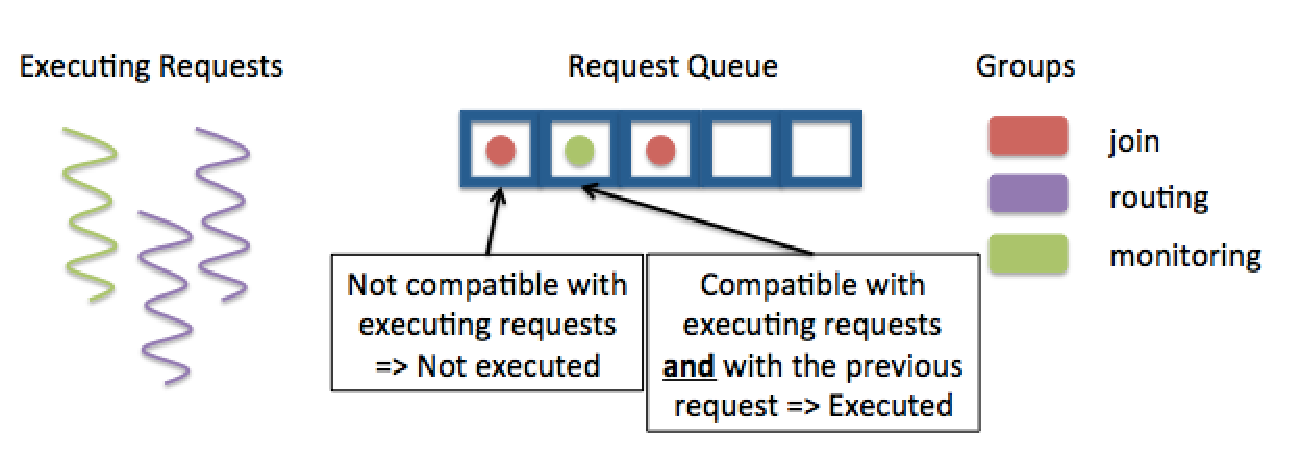
\includegraphics[scale=0.5]{pictures/multiactive_object.pdf}
      \end{minipage}
      \caption{First compatible first out policy of multiactive objects}
      \label{fig:multiactive_object}
\end{figure}

\subsection{Request service mechanism of multiactive objects}\label{sec:MAOservice}
At any time, each ready-to-execute request should be assigned an execution thread. But to avoid killing the whole performance by creating too many threads on the fly, the number of threads that can be run at the same time can be limited. This limit can be set directly in the code. In this case, multiactive objects rely on a fixed thread pool to execute ready requests.  
As a consequence of this limit, even requests that are ready to execute (i.e. that are compatible) might wait in the queue if all available threads are busy. Those requests that are ready to execute but that cannot be executed because of lack of threads form a new queue that we will call \emph{ready queue}. 
Schematically, when a new request comes to an multiactive object, it is put in the \emph{reception queue} of the multiactive object. Then, the compatibility filter is applied to select only the requests that are compatible, according to the policy describe earlier. Once filtered, those requests are put in the ready queue, waiting that some thread is freed to execute. In fact, the reception queue holds incompatible requests whereas the ready queue holds compatible requests. Each requests must go through both queues to be executed, since the scheduling of requests occurs at the head of the ready queue. This mechanism is pictured on Figure~\ref{fig:queues}.

\begin{figure}[ht]
      \begin{minipage}[c]{\textwidth}
      \centering
      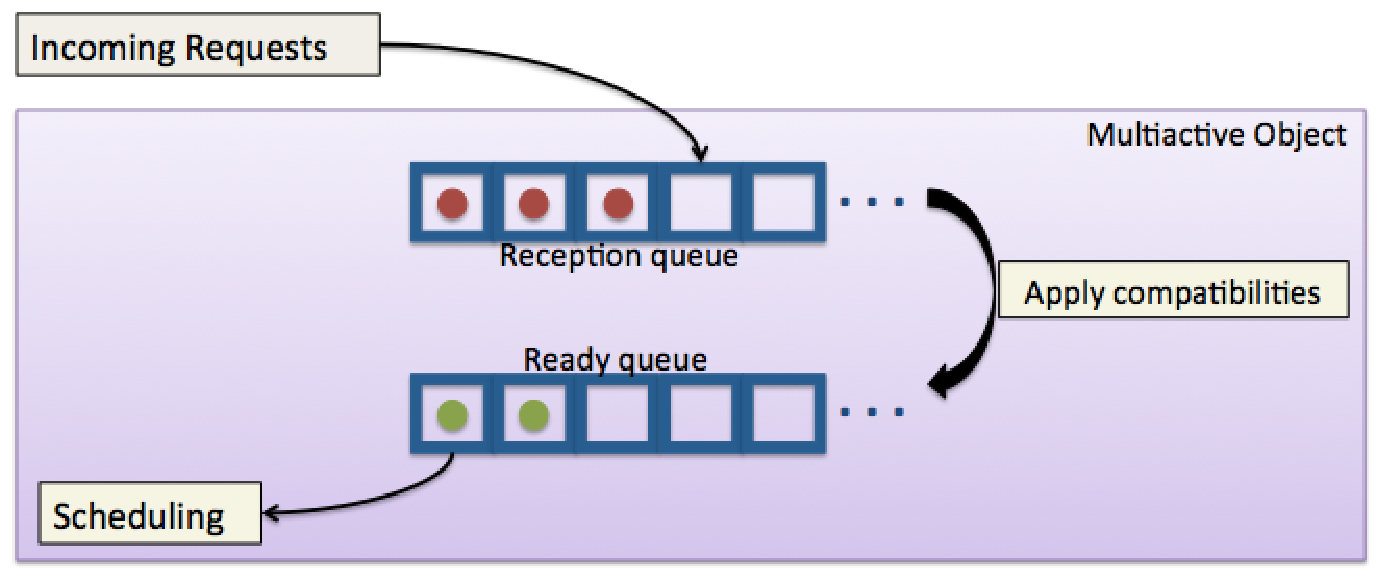
\includegraphics[scale=0.5]{pictures/queues.pdf}
      \end{minipage}
      \caption{The different queues operating in a multiactive object}
      \label{fig:queues}
\end{figure}

Considering the thread limitation, working on the ready queue and improve request scheduling is necessary to optimize request executions according to the programmer's needs. Indeed, introducing scheduling mechanisms at the reception queue level is useless since it is the compatibilities that first decide if a request is ready to be executed. For those reasons, all the objectives described below apply on the ready queue only.

\subsection{Internship Objectives}
The internship takes place in the context of multiactive objects. The main objective of the internship is to enhance the multiactive object programming model, by offering to the programmer more control on the scheduling of requests. To achieve this goal, we want to propose a priority mechanism applied to multiactive objects, in order to sort the requests in the ready queue according to their importance. We also want the programmer to be able to influence the scheduling of requests by setting limits on the number of threads that a type of request can occupy at the same time. The motivation here is to increase the efficiency of multiactive objects in the sense that the programmer will be able to favor processing of requests that are of most importance, while keeping a maximum parallelism and a safe execution.
In particular, here are the main steps of the expected achievements:

\begin{enumerate}
\item Design, implement and analyze several priority specifications. The goal is to design a priority specification that is at the same time:
	\begin{itemize}
	\item \textbf{User-friendly} \\The request priorities must be easy to define for the programmer and also easy to maintain (even with a high number of priorities to specify).
	\item \textbf{Expressive} \\Any kind of priority dependency must be covered by the priority specification.
	\item \textbf{Consistent} \\with the existing programming model, basically, using meta programming.
	\item \textbf{Effective} \\The scheduling policy must take into account priorities as much as possible.
	\item \textbf{Efficient} \\The priority specification must introduce a minimal additional cost to the execution of the scheduling policy.
	\end{itemize}
\item Design and implement mechanisms to manage thread allocation. Propose tools for the programmer to be able to:
	\begin{itemize}
	\item Set the size of the thread pool.
	\item Reserve some threads for particular requests. \\This tool can be used to specify that high priority requests have threads only devoted to them: this is a way to avoid the priority inversion problem.
	\item Set a maximum limit on the number of threads that can be used by particular requests at the same time. \\A good usage of this tool will ensure that low priority requests are not starved, i.e. all requests in the queue are eventually executed.
	\end{itemize}
\item Experiment the previous mechanisms through usecases in order to:
	\begin{itemize}
	\item Show that the priorities help to have a better throughput of most important requests: the priority mechanism is successfully applied.
	\item Ensure that the priority mechanism does not have a too big overhead: the time to choose the next request to execute according to priorities must be reasonable.
	\end{itemize}
\end{enumerate}

Implementation of the proposed features will be done directly in the current implementation of multiactive objects, that is in the latest version of the Proactive Java middleware \cite{ref:proactive}.
The OASIS research project-team is currently involved in a European project \cite{ref:play} that deals with automatic notification delivery through peer-to-peer networks using a Publish/Subscribe mechanism. This system is currently implemented using multiactive objects. Achievements of this internship objectives will contribute to improve the performance of this system. Experimentations will be carried out in this system, as it provides facilities to deploy multiactive objects.  

The main challenge in this work is to find the most efficient specification that will improve expressiveness of multiactive objects, while keeping the model convenient for the programmer. In particular, finding the right balance between all the given parameters is the most tricky part, and experimental evaluations should corroborate design choices.

\section{Related works}
In this section we review works that have been done in the domain of concurrency models or scheduling policies, in order to facilitate access to parallelism or to raise scheduling concerns at the application level.
\subsection{JAC}
JAC (Java with Annotated Concurrency) \cite{ref:jac} is an extension of the Java language that aims to separate concurrency constructs from the application logic. JAC proposes a set of annotations that allow the programmer to specify whether the annotated entity must be guarded by a lock or if it can be run concurrently by several threads. This simplifies concurrency for non experimented programmers in this domain. More precisely, annotations are processed at precompile time (which limits runtime resolved decisions) and \textbf{synchronized} Java keywords are then introduced where needed before compilation. Most of the given annotations and facilities offered by JAC are very close to the ones offered by multiactive objects, especially to define method compatibility. However, in multiactive objects, as the annotations for compatibilities are checked at runtime, compatibilities can be defined depending on the value of the request parameters, which cannot do JAC since its annotations are evaluated at precompile time.

In addition to compatibilities, JAC proposes a \textbf{@schedule} annotation, placed on top of a method, that allows the programmer to define a boolean method (linked to the annotated method) to decide whether the annotated method can be executed when invoked, in addition of compatibility rules. In this boolean method, the list of waiting requests is accessible, which makes possible to define fine-grained scheduling policies.
However, this way to influence scheduling of request is fairly complex, as it requires that the programmer directly manipulates the requests in the queue. Unlike JAC, we want to offer very high level and intuitive scheduling mechanisms.


\subsection{Scheduling in ABS}
Although the ABS language (see Section~\ref{sec:ABS}) offers by default no deterministic policy to execute ready requests, ABS still proposes to write user-defined schedulers that can be translated into Maude language (but not into Java), to override the non deterministic default policy. Thus, the programmer can define several customized schedulers and then specify one of them to be used in a particular cog. User-defined schedulers are methods written in the ABS language and they can be used through the \textbf{scheduler} ABS annotation that must mention the scheduler method name. More precisely, a user-defined scheduler method must select a request to execute among a list of requests waiting for a given object. As in ABS requests contain a lot of information (arrival date, waiting time, method call name, crucial method flag etc...), it is easy to design a customized scheduling policy based on any kind of criteria. 

But there are two problems in this design according to our objectives. Firstly, a user-defined scheduler has not the last word about which request is actually executed: user-defined schedulers choose one request among waiting requests of a given object. But then, it is the cog that non deterministically decides which object is allowed to execute its requests. So in the end, schedulers have only a partial impact on the scheduling. So firstly, this violates our objective to have an effective user-defined scheduling. Secondly, user-defined schedulers in ABS still constrain the programmer to write code that manipulates the queue, which violates our user-friendly objective too.


\subsection{Application-level scheduling in Creol}
In this work~\cite{ref:Nobakht:2012:PDA:2245276.2232086}, the authors extend the Creol  language (Section~\ref{sec:Creol}) by introducing an application-level scheduling which relies on request priorities. Initially, in Creol, requests that are in the queue or that are waiting to resume are selected for execution in a non deterministic manner. This extension override this non deterministic behavior by assigning a priority to requests. Each request has either a user-defined priority, or a default priority, materialized by an integer. The lower the integer is, the higher the priority is. 

More precisely, the priorities of requests are assigned in two steps. First, a Creol active object interface must define a range of priority values. Second, when a method call is performed on an active object, the caller may assign a priority value in the range defined by the interface of the active object. Also, as the client side might always ask for the highest priority, the server side can also set a fixed priority value. So request priorities can be defined both on the server and client side. Then, to decide the final priority of a particular request, the active object applies a deterministic function that takes into account both the method call priority and the request definition priority.

Although this work is very interesting as it provides a high level scheduling hints, it is still complex to use because the programmer does not know right away the priority value of a request, because of server and client priority values, and because of the function that is applied on them. In our approach, we chose to assign priorities only on the server side, for the programmer to better visualize the priorities that will be actually applied. 


\subsection{Positioning}
Regarding related works about request scheduling, JAC gives the possibility to impact on the execution of requests by letting the programmer define particular methods on top of requests, to decide their scheduling. Those methods are called just before trying to execute the request, to decide if it should actually be executed. ABS proposes a similar mechanism, known as user-defined schedulers, which are functions that manipulate the queue to select the request to execute. Although those solutions can provide a fine-grained selection of requests, because the programmer directly manipulates the queue, they are too low-level and they imply to write a significant part of the scheduling code. In our work, we prefer to provide mechanisms based on specification (not involving too much user-defined scheduling code), as they are more high-level and easier to use. 

On the other hand, Application-level scheduling in Creol, which is the closest work to ours, provides request priority assignment, using a high level declaration language. Priorities can be assigned both on the client and server side, for fairness reasons, and then a deterministic function combines all priorities to guess the final one. This offers a very precise control of request execution. However, we consider that it is too complex because whenever the programmer assigns priority values, he has to be aware of all the values previously defined on both sides. He does not know right away the real priority value. In our work, we try to make the priority mechanism the easiest to use for the programmer. We want to keep both simplicity and expressiveness.

It is worth noticing that no related work considers at the same time distribution and true concurrency. Indeed, JAC provides no facilities for distribution and ABS and Creol provide no parallelism of requests, just interleaved executions. On the other hand, multiactive objects provide distribution (via active objects) and true parallelism of requests. Therefore, in addition of request execution order, we also give in this work scheduling tools to manage the parallelism in a programming model that is at the same time globally distributed and locally concurrent.

\chapter{Contributions}\label{sec:contributions}
In this chapter, we present contributions to the multiactive objects model, regarding mainly priority of requests, thread management, and their validation through experiments.

\section{Design and implementation of scheduling controls}
\subsection{Priority specifications}
\subsubsection{Introduction}
The multiactive object model enables multi-threading within an active object. While this model is convenient for completing multiple requests at the same time, it does not enable a particular scheduling other than First Compatible First Out, as introduced in Section~\ref{sec:MAOprinciples}. But the programmer might appreciate some requests to be executed before some others if possible, that is, express a \emph{priority} relationship between the requests. 
We can define priority relationship as the fact to reorder the requests in the queue such that a request which has a high priority can overtake requests which have a low priority. 
The main objective here is to reduce response time of most important requests. 

Currently, in multiactive objects, requests lie in the reception queue in the order they have been received, that is a First In First Out ordering. Requests in the reception queue are then filtered such that compatible requests are pulled out to lie in a new queue that we call ready request queue, as explained in Section~\ref{sec:MAOservice}. Requests are then executed according to the order of the ready queue. In the ready queue, a request is always placed after older requests and before more recent requests. Therefore, if in the ready queue a very important request is placed after a lot of unimportant requests, then the very important request has to wait the completion of all the unimportant requests before being processed. Prioritizing requests at the ready queue level aims at solving this problem by executing most important requests first, and this is what we introduce in this work. Criteria of importance can be of multiple sources. For example, in a storage system where updating the content is critical, we would like to be able to postpone reading requests after modifying requests. Assuming that we are using an object as front end to store and retrieve content in this system, Figure~\ref{fig:priority_principle} displays what could happen in this case with prioritized requests:

\begin{figure}[ht]
      \fbox{
      \begin{minipage}[c]{\textwidth}
      \centering
      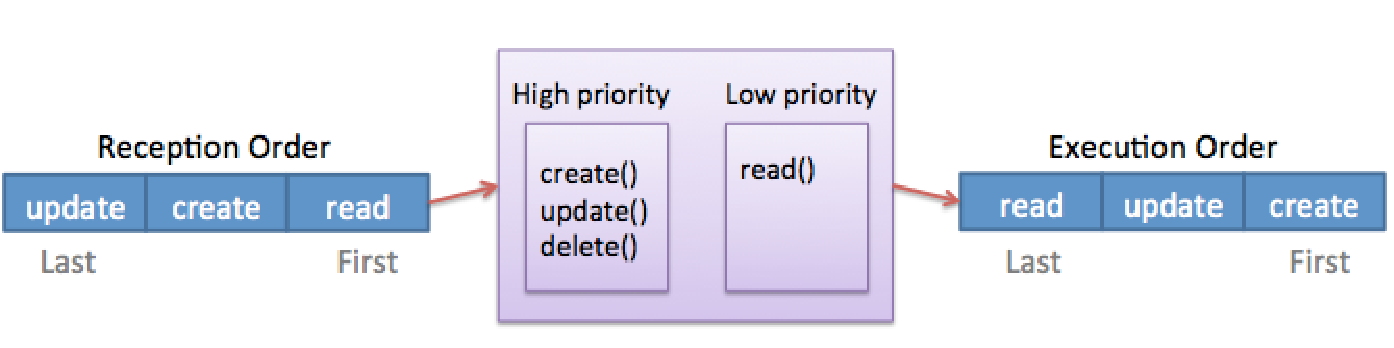
\includegraphics[scale=0.5]{pictures/priority_principle.pdf}
      \end{minipage}
      }
      \caption{Principle of priorities: reorder request execution}
      \label{fig:priority_principle}
\end{figure}

In this example, there are four exposed requests: \textbf{create}, \textbf{read}, \textbf{update} and \textbf{delete}. Those methods are partitioned into two groups (that we assume compatible with each other): the first one has a high priority and the second one has a low priority. Suppose that three requests are received for execution: first \textbf{read}, then \textbf{create}, and finally \textbf{update}. As we declared that the \textbf{read} request has the lowest priority, it is processed last, even if it was received first. It is this principle of priority that we want to address particularly in multiactive objects.

\paragraph{}
As we have seen in Section~\ref{sec:MAOprinciples} a particular language has been designed using the JAVA annotation mechanism in order to allow the programmer to define compatibilities of requests. We have used the same kind of mechanism to offer to the programmer the possibility to define request priorities, to remain consistent with the existing framework. For that, in addition to the compatibility annotations, we have created new Java annotations for priorities. Those new annotations should also be located on top of a multiactive object class definition, and they should apply on request that the multiactive object defines. 
Priority annotations are then processed by the priority annotation handler that we have also developed, to adapt the scheduling of requests according to the defined priorities.

This results in a new simple declarative language that the programmer can use in order to easily assign priorities to requests. More precisely, we have chosen to assign priorities to groups instead of requests, because compatibilities apply also to groups. Therefore, we keep the group granularity which is more general, still in our objective of being consistent with the existing programming model. As a consequence, all requests of the same group have the same priority. This does not restrict the possibilities of the mechanism: a group can still be split into several groups if needed.
Note that, despite the fact that our particular implementation is described in the following, this priority model is not tight to a particular implementation of active objects. Indeed, it can be implemented in any programming language that supports meta programming.

In the following sections, we review two kinds of priority specification. The first specification is based on integer assignment and the second one is based on a dependency graph. We will analyze those specifications in order to converge towards a specification that meet most of the objectives we expect. Both specifications use customized annotations that we have developed in the current multiactive object implementation. 

\subsubsection{Integer-based priority specification}
Integer assignment is a classical approach to deal with priority, mainly at the operating system level, but also at most of application-level scheduling systems. Integer assignment consists in associating an integer to a process/request/task, or more generally to entities to prioritize. Thanks to this association, entities can then be ordered by importance, according to the meaning of the integers.

At the request level, integer assignment determines execution order of requests. As it is a classical approach to implement priorities, we have adapted this specification to our model. In our case, we want to assign a priority value to requests of a given group. For that, we have developed two new annotations. The first one is called \textbf{@DefineIntegerBasedPriorities}. This global annotation is meant to contain several \textbf{@Priority} annotation entries. One \textbf{@Priority} entry corresponds to one level of priority. It accepts two attributes: first, names of groups previously defined, and second, level of priority, materialized by an integer. Several groups can be given the same level of priority. Figure~\ref{integer_priority_annotation} is an example of how our annotations are used to assign priorities to groups in the Java source, on top of a multiactive object class:

\begin{figure}[!ht]
	\lstset{language=java, numbers=left, numberstyle=\tiny, stepnumber=1, numbersep=5pt, basicstyle=\footnotesize}
	\begin{lstlisting}[frame=single]
@DefineIntegerBasedPriorities({
  @Priority(groupNames = {"G1"}, level = 5),
  @Priority(groupNames = {"G2", "G3"}, level = 3),
  @Priority(groupNames = {"G4"}, level = 2)
})
 	\end{lstlisting}
\caption{An example of priority annotations based on integer assignment}
\label{integer_priority_annotation}
\end{figure}

Here, four groups are given a priority, named \textbf{G1}, \textbf{G2}, \textbf{G3}, and \textbf{G4}. The highest priority requests are the ones of group \textbf{G1}, because it is assigned the highest value. Thus, in this example, requests of group \textbf{G1} will be the first to be allocated a thread if they are ready to be served. Requests of groups \textbf{G2} and \textbf{G3} share the same level of priority and have a lower priority than group \textbf{G1}. Finally, requests of group \textbf{G4} have the lowest priority. Thus, if requests of those groups are in the ready queue at the same time, they will be ordered according to their priority value: requests of group \textbf{G1} will be firsts, and requests of group \textbf{G4} will be lasts.
Of course, we suppose here that all the groups mentioned in a \textbf{@Priority} annotations are previously declared in a \textbf{@Group} annotation. 

The advantage of this priority specification is that it is simple  to process. Knowing whether a request can be executed before another one consists in three steps:

\begin{enumerate}
\item Look up group membership of the request
\item Look up the group priority value
\item Compare the value with others in the queue and position the request accordingly
\end{enumerate}

So the main operation to decide on the position of a request in the ready queue is integer comparison. This operation is fast, since comparing two integers is fast. This is another advantage of this specification: it should have a good performance in practice as the priority processing should be here very fast. In our case, a good performance means a low overhead.

For requests of groups that do not have a priority value, an arbitrary default value is given. As well, requests that do not belong to any group have also a default priority value. In our implementation, the default value given is 0, and this value it is not customizable. 

Note that a request that does not belong to any group cannot have a user defined priority since priorities require group names. In the end, all requests have a priority value, even if they do not belong to any group nor have any priority. As all requests have a priority value, we can always compare them to each other. Therefore, we can always order requests. If two requests have the same priority value, then we order them following a FIFO policy. As a consequence of those two rules, we can always order requests in a strict total order.
The insertion process of requests in the queue is the following. For all incoming request R group G, considering a ready queue composed of $R_1,R_2,...,R_n$ belonging to groups $G_1,G_2,...,G_n$, $R$ is  inserted in just before the lowest $R_i$, $i \le n$, such that the priority value of G is greater than the priority value of $G_i$, if such a $R_i$ exists. Else, it is inserted after $R_n$.
More formally, we can define the insertion process as defined below:
\paragraph{Insertion process}
$group(R)=G' \wedge Q=[R_1,...,R_n] \wedge \forall i \in 1,...,n$, $group(R_i)=G_i$
\begin{itemize}
\item $if$ $priority(G_n) < priority(G)$,\\$let$ $j=min({i| priority(G_i) < priority(G)})$, $insert(R, Q)=[R_1,...,R_j_-_1,R,R_j_+_1,...,R_n]$
\item $else$ $insert(R,Q)=[R_1,...R_n,R]$
\end{itemize}

\subsubsection{Limitations of the integer-based priority specification}
Always ordering the requests in a total order can be a drawback. Even if the programmer does not assign a priority to all the groups, all requests are tight with an order relation. But sometimes requests are not related at all, and there is no reason that one overtakes another in the queue. In this case we would like to keep the \emph{unrelated} relationship. As an example, consider the priority definition of Figure~\ref{fig:two_priorities}:

\begin{figure}[!ht]
	\lstset{language=java, numbers=left, numberstyle=\tiny, stepnumber=1, numbersep=5pt, basicstyle=\footnotesize}
	\begin{lstlisting}[frame=single]
@DefineIntegerBasedPriorities({
  @Priority(groupNames = {"G2"}, level = 2),
  @Priority(groupNames = {"G1"}, level = 1),
})
 	\end{lstlisting}
\caption{A priority relation involving two groups}
\label{fig:two_priorities}
\end{figure}

Group \textbf{G2} has a higher priority than group \textbf{G1}. Aside, we want to specify that \textbf{G3} is not related with \textbf{G2} nor \textbf{G1}. However, with integer assignment, requests of group \textbf{G3} will always have either to wait after requests of at least one group or to overtake requests of at least one group, whatever the priority value assigned to it. This is inconvenient because this priority value will inevitably affect the throughput of requests of group \textbf{G2} and \textbf{G1}, whereas we want \textbf{G3} to be unrelated to them. Thus we cannot express the unrelated relationship using integer assignment.   
In this sense we can say that this priority specification language is not expressive enough to cover any usage. 

Another drawback of this specification is that it is not user-friendly enough in our sense. Indeed, assigning a priority value to a new group implies to remember previously assigned values for groups we want to overtake. Removing this indirection will allow the priority specification to be expressed more clearly. Instead, we expect a specification where the programmer simply says that he wants group to have priority over another group, without relying on additional knowledge.

This integer-based priority specification lacks of expressiveness and user-friendlyness. Those are the two reasons why we moved to another specification to define request priorities, that is more expressive and user-friendly. We describe this new specification in the next section.
 
\subsubsection{Graph-based priority specification}
In order to overcome the drawbacks of integer-based priority specification, we developed a second model based on a dependency graph. The motivation of this specification is that it is able to express a relative relationship between groups instead of relying on absolute values. The idea is to implicitly define priority dependencies through the annotation itself, not through its attributes. Then, the annotations are processed in order to build a dependency graph, where nodes contain groups and edges represent a priority relation. This way, the internal representation of priorities is not exposed to the user, making the annotations higher level, and therefore, easier to use.

The new annotations we have developed are based on the following structure. First, a \textbf{@DefineGraphBasedPriorities} annotation is in charge of containing several dependency trees. Each of them is defined in a \textbf{@PriorityOrder} annotation. A \textbf{@PriorityOrder} annotation contains the groups, in an ordered manner using \textbf{@Set} annotations, such that each upper line represents a priority dependency to the lower line. As a simple example, Figure~\ref{graph_priority_annotation} displays the same configuration as the previous one depicted using integer-based priorities:

\begin{figure}[!ht]
	\lstset{language=java, numbers=left, numberstyle=\tiny, stepnumber=1, numbersep=5pt, basicstyle=\footnotesize}
	\begin{lstlisting}[frame=single]
@DefineGraphBasedPriorities({
  @PriorityOrder({
    @Set(groupNames = {"G1"}),
    @Set(groupNames = {"G2", "G3"}),
    @Set(groupNames = {"G4"})
  }),
})
 	\end{lstlisting}
\caption{Graph-based priority annotations}
\label{graph_priority_annotation}
\end{figure}

Here, no value nor particular indication are given. It is only the order in which the groups are defined that is significant. Specifically, there is a priority dependency from \textbf{G1} to \textbf{G2} and \textbf{G3}, and from \textbf{G2} to \textbf{G4} and \textbf{G3} to \textbf{G4}.

Internally, when processed, this priority definition is stored as a dependency graph pictured on Figure~\ref{fig:graph}:

\begin{figure}[!ht]
      \fbox{
      \begin{minipage}[c]{\textwidth}
      \centering
      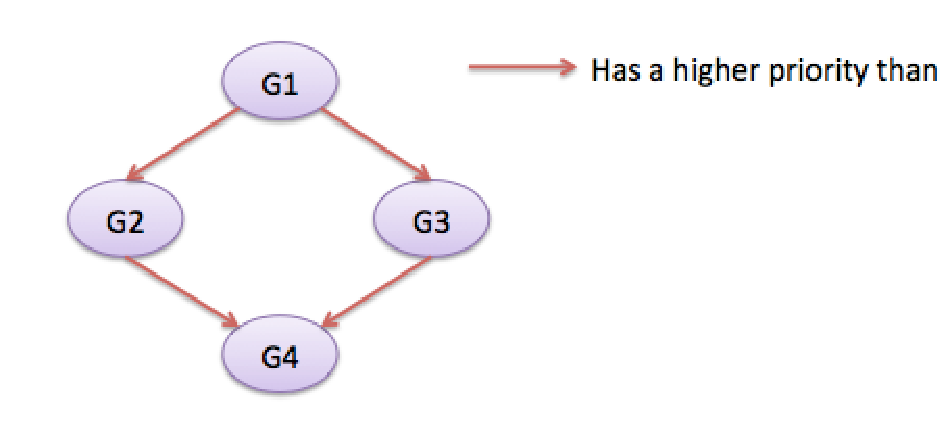
\includegraphics[scale=0.5]{pictures/graph.pdf}
      \end{minipage}
      }
      \caption{Dependency graph corresponding to the definition of Figure~\ref{graph_priority_annotation}}
      \label{fig:graph} 
\end{figure}

This example can be defined using only one \textbf{@PriorityOrder} annotation. But the advantage of the graph-based priority specification is that we can define several branches of the graph separately without impacting the whole meaning. Figure~\ref{graph_priority_definition_2} shows another example of the same graph definition:

\begin{figure}[!ht]
	\lstset{language=java, numbers=left, numberstyle=\tiny, stepnumber=1, numbersep=5pt, basicstyle=\footnotesize}
	\begin{lstlisting}[frame=single]
@DefineGraphBasedPriorities({
  @PriorityOrder({
    @Set(groupNames = {"G1"}),
    @Set(groupNames = {"G2"}),
    @Set(groupNames = {"G4"})
  }),
  @PriorityOrder({
    @Set(groupNames = {"G1"}),
    @Set(groupNames = {"G3"}),
    @Set(groupNames = {"G4"})
  }),
})
 	\end{lstlisting}
\caption{Another way to define the graph depicted on Figure~\ref{fig:graph}}
\label{graph_priority_definition_2}
\end{figure}

In fact, one \textbf{@PriorityOrder} annotation corresponds to a linear representation of graph paths. With this specification, we can define the same priorities in different ways, according to the groups we want to focus on.

In the previous example, both the meaning and the impact of the priority definitions is exactly the same as the one defined with integer-based specification. And indeed, an integer-based priority specification can always be translated into a graph-based specification. However, a dependency graph cannot always be translated into a integer-based specification, because of the \emph{unrelated} relation. Indeed, the unrelated relation is covered by the graph specification but not by the integer specification. Consider this particular dependency graph displayed on Figure~\ref{fig:graph_2}:

\begin{figure}[!ht]
      \fbox{
      \begin{minipage}[c]{\textwidth}
      \centering
      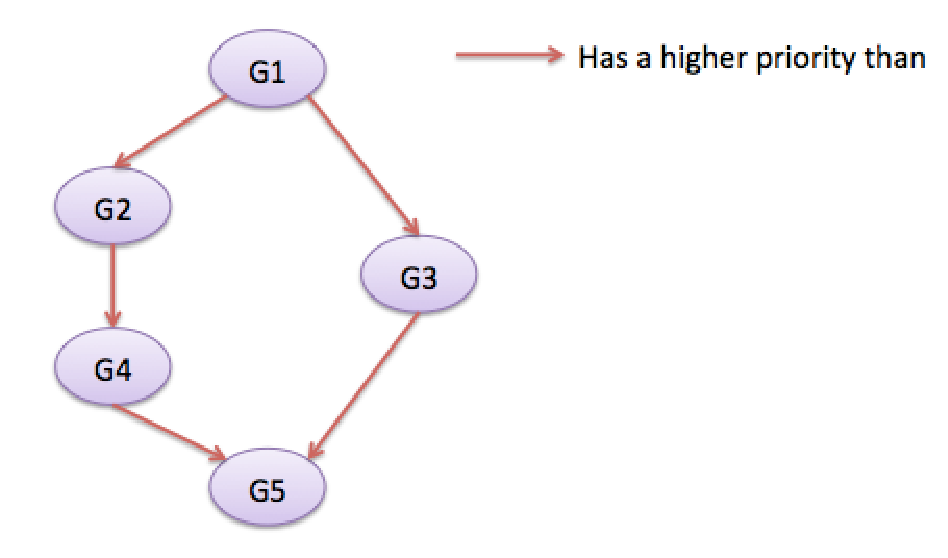
\includegraphics[scale=0.5]{pictures/graph_2.pdf}
      \end{minipage}
      }
      \caption{Dependency graph that cannot be translated with integer assignment}}
      \label{fig:graph_2} 
\end{figure}

In this graph, there are two unrelated relations. In particular, \textbf{G3} is not related with \textbf{G2}, and \textbf{G3} is not related with \textbf{G4}. This is perfectly definable using our graph-based specification, by defining the two branches in separate \textbf{@PriorityOrder} annotations, as defined on Figure~\ref{fig:new_priority_annotation}:

\begin{figure}[!ht]
	\lstset{language=java, numbers=left, numberstyle=\tiny, stepnumber=1, numbersep=5pt, basicstyle=\footnotesize}
	\begin{lstlisting}[frame=single]
@DefineGraphBasedPriorities({
  @PriorityOrder({
    @Set(groupNames = {"G1"}),
    @Set(groupNames = {"G2"}),
    @Set(groupNames = {"G4"}),
    @Set(groupNames = {"G5"}),
  }),
  @PriorityOrder({
    @Set(groupNames = {"G1"}),
    @Set(groupNames = {"G3"}),
    @Set(groupNames = {"G5"})
  })
})
 	\end{lstlisting}
\caption{Relative priority annotation}
\label{fig:new_priority_annotation}
\end{figure}

However, this cannot be defined using integer assignment. Indeed, what value should be assigned to \textbf{G3} in order to not always overtake (or respectively, to not always be overtaken by) \textbf{G2} nor \textbf{G4}? This idea is impossible to express with the integer-based specification.
In the same idea, with the graph-based specification, there can exist \textbf{@PriorityOrder} annotations that lead to a disconnected graph. It is exactly what we want to be able to express, as to be able to express unrelated groups. To summarize, here are the points that have been enhanced thanks to the graph-based specification: 

\begin{itemize}
\item \textbf{More expressive}\\ The set of priority relationships that can be expressed with the graph-based specification is larger than the set of priority relationships that can be expressed with the integer-based specification, and the whole set of integer-based specifications is included in the set of graph-based specifications.
\item \textbf{Easier to use}\\ Branches of the graph can be defined separately, which makes the model more scalable. Even with a high number of user-defined priorities, more priorities can still be added easily without taking into account the existing set of priorities.
\end{itemize}

\subsubsection{Graph properties}
We have seen that the graph-based priority specification has more advantages than the integer-based priority specification. We are going now to expose properties of our dependency graph that are essential to understand the scheduling policy.\\

\textbf{Notations}\\
Firstly, let us introduce the notations that will be used in the following paragraphs. 
\begin{itemize}
\item We start from a dependency graph defining a priority relation between groups, denoted with the operator $\longrightarrow$.
\item In the graph, reachability is denoted with the $\longrightarrow^{+}$ operator that has two operands. The $\longrightarrow^{+}$ operator means that the second operand can be reached from the first one, i.e. that there exists a directed path from the first operand to the second one. The $\longrightarrow^{+}$ operator is called the \emph{transitive closure} of the $\longrightarrow$ operator.
\item In our context, $G_1$ $\longrightarrow^{+}$ $G_2$ means that group $G_1$ has a higher priority than group $G_2$, since $G_2$ is reachable from $G_1$ in the directed dependency graph.
\item A request is generally denoted $R$, a group denoted $G$ and the queue denoted $Q$.
\end{itemize}\\

\textbf{Absence of cycles}\\
The dependency graph is inferred from the programmer's annotations. Thus, it is possible that the programmer, consciously or not, creates cycles in the dependency graph. For example, Figure~\ref{fig:cycle} is a  syntactically correct priority declaration, but it creates a cycle that indefinitely goes from $G_1$ to $G_2$ and from $G_2$ to $G_1$.

\begin{figure}[!ht]
	\lstset{language=java, numbers=left, numberstyle=\tiny, stepnumber=1, numbersep=5pt, basicstyle=\footnotesize}
	\begin{lstlisting}[frame=single]
@DefineGraphBasedPriorities({
  @PriorityOrder({
    @Set(groupNames = {"G1"}),
    @Set(groupNames = {"G2"})
  }),
  @PriorityOrder({
    @Set(groupNames = {"G2"}),
    @Set(groupNames = {"G1"})
  })
})
 	\end{lstlisting}
\caption{An example of priority definition that leads to a dependency cycle}
\label{fig:cycle}
\end{figure}

Unchecked cycles in the dependency graph would lead to never ending search at some point, for example, infinite search of optimal position when inserting a new request. In order to prevent abnormal behavior related to graph cycles, we have enhanced our previous graph construction process. At each new annotation line encountered, we check if the new dependency will lead to a cycle in the graph. If so, the dependency is not created. If the node currently considered did not exist already, then it is not created either. Following annotation lines are still taken into account if the mentioned node existed before. In case of a detected cycle in the annotations, an error message is displayed showing the incriminated dependencies. Thus, by construction, we ensure that there is no cycle in the dependency graph we build. More precisely, we can classify our dependency graph as a Directed Acyclic Graph (DAG) \cite{ref:gallai1968directed}.\\

\textbf{Unicity}\\
In our dependency graph, each group belongs to a single node. We ensure this fact by construction too: when a group name is encountered in a priority annotation, the algorithm first searches a node whose group has the same name. If such a node exists already in the graph, then no additional node is created. Only the references that point towards higher priority nodes and lower priority nodes are updated. When a new node is created because it does not exist already, the new node is stored such that it can be retrieved (by exploring the graph) if it is referenced later.\\

\textbf{Overtakability}\\
In our scheduling objective, the main information we want to extract from the graph is whether a request can overtake another one. More generally, as we operate on groups of requests, we are interested in knowing whether a group has a higher priority than another one. This information lies in the dependency graph.
\begin{itemize}
\item A request of group $G_1$ can overtake a request of group $G_2$ if and only if $G_1\longrightarrow^{+}G_2$, i.e. if it exists a directed path from $G_1$ to $G_2$.
\item A request of group $G_1$ has no priority relation with a request of group $G_2$ if (\lnot~\ $G_1\longrightarrow^{+}G_2$)~\ \wedge~\  (\lnot~\ $G_2\longrightarrow^{+}G_1$), i.e. if there is no directed path from $G_1$ to $G_2$ and no directed path from $G_2$ to $G_1$. In this case we say $G_1$ // $G_2$.
\end{itemize}
Considering our insertion policy described below, what is important from those definitions is that $G_1$ cannot overtake $G_2$ if either $G_1$ // $G_2$ or $G_2\longrightarrow^{+}G_1$.\\

\textbf{Insertion}\\
In practice, when a new request is received and must be inserted in the priority queue, overtakability properties are used to determine the position of the new requests according to the priorities.
In particular, an incoming request of group $G$ must be inserted in the priority queue just before the first request whose group can be overtaken by the group of the inserted request. Precisely, 
considering $R$ of group $G$ to be inserted in Q, and
$Q$ = $R_1,R_2,...,R_n$ of groups $G_1,G_2,...,G_n$, then $R$ is inserted just before the smallest $R_i$, $1 \le i \le n$, such that $G\longrightarrow^{+}G_i$, or at the end of the queue if~\ \forall $j$,~\ $1 \le j \le n$,~\ \lnot~\ $G\longrightarrow^{+}G_j$ .\\
More formally, we can define the insertion process as defined below:
\paragraph{Insertion process}
$group(R)=G' \wedge Q=[R_1,...,R_n] \wedge \forall i \in 1,...,n$, $group(R_i)=G_i$
\begin{itemize}
\item $if$ $\forall$ $i$ \lnot $G\longrightarrow^{+}G_i$,$insert(R,Q)=[R_1,...R_n,R]$
\item $else$ $let$ $j=min({i|G\longrightarrow^{+}G_i})$, $insert(R, Q)=[R_1,...,R_j_-_1,R,R_j_+_1,...,R_n]$
\end{itemize} 

\newtheorem{insertion}{Theorem}
\begin{insertion}
A request must be inserted just before the first request it can overtake.
\end{insertion}
\begin{proof}[Proof]
Let us prove by contradiction that the insertion policy is correct regarding the priority specification.
Suppose that it exists a request $R_j$ positioned after  
$R_i$ in the queue such that $R$ can overtake $R_i$, but cannot overtake $R_j$ (i.e. $\LB{G}\longrightarrow^{+}\LB{G_i}$ and  $\LB{G_j}\longrightarrow^{+}\LB{G}$). Then it means that we have $\LB{G_j}\longrightarrow^{+}\LB{G}\longrightarrow^{+}\LB{G_i}$. So by transitivity, we would have $\LB{G_j}\longrightarrow^{+}\LB{G_i}$,
which is contradictory with the fact that $R_i$ positioned before $R_j$ means $\LB{G_i}\longrightarrow^{+}\LB{G_j}$. So there is no request positioned after $R_i$ that has a higher priority than $R$. As a consequence, it is correct to insert $R$ just before $R_i$.
\end{proof}[]
%\[\begin{aligned}
%\end{aligned}\]

\paragraph{}
To conclude, the graph-based priority specification is very convenient to define relative priorities between group of requests of multiactive objects. The programmer only defines dependencies between groups, that are then automatically taken into account as priorities when scheduling requests. This specification internally uses a customized dependency graph that is not visible from the user. This allows our graph to have strong properties. The only drawback of this specification is that it uses a quite complex structure (a graph) that (1) has to be kept in memory the entire execution time, and (2) might be entirely explored each time a request is inserted in the ready queue. The second point indirectly impacts on the scheduling time of requests since the queue must be locked during the insertion process to prevent data races. This can be a problem relatively to our objective of efficiency, which stipulate that our priority specification should have a low overhead on the scheduling time. On the other hand, the integer-based specification seems to be well adapted for efficient processing. This is why, despite the convenience of the graph-based specification, we need to validate this specification through experiments that compare it with the integer-based specification. Such experiments will be presented in Section~\ref{sec:experiments}.

Note that from Java version 8 (that is not yet released - planned on early 2014), we will be able to get rid of the container annotations. In our implementation of priority specifications, container annotations are named with the \textbf{@Define} prefix, as in \textbf{@DefineIntegerBasedPriorities} and \textbf{@DefineGraphBasedPriorities}. Indeed, Java 8 will introduce the possibilty to use an annotation more than once on top of a given entity, which is not allowed for the moment. This is why we relied on container annotations to encapsulate several declarations, which makes the priority specification a little bit heavier.

\subsection{Thread management}
\subsubsection{Introduction}
We increased control of scheduling of requests in multiactive objects by offering to the programmer a powerful priority specification. But to offer further control on the scheduling we also provide a mechanism to manage threads that are available to execute the requests. Indeed, the way the threads are allocated to execute the requests is not customizable in multiactive objects. As soon as a requests is selected for execution, it is allocated the first available thread. In particular, no further checking is made about requests already executing, nor about waiting requests. The problematic is the following: considering that we have a limited number of threads and that we have also introduced priorities to execute requests, then abnormal situations can arise. Especially, low priority requests can suffer of \emph{starvation}. Starvation is a condition where access to a resource is perpetually delayed such that it will never be accessed. In our context, the resources are threads, and the entities that fight to access the threads are requests. For example, a starvation situation can occur in our case when a continuous stream of requests of high priority comes, preventing low priority requests from being executed. 
This part of the work aims at being able to partition the threads among the different groups (i.e. to the different priority levels) according to the programmer's wish. 

\subsubsection{Starvation of low priority requests}
To prevent starvation of low priority requests at the programming level, we have enhanced the existing group definition. The goal is to allow the programmer to set a limit on the number of threads that requests of a particular group can use at a time. Optionally, the \textbf{@Group} annotation can now declare an attribute that determines the maximum number of threads that requests of the group can occupy at the same time. Figure~\ref{fig:new_groups} displays an example of the new group annotation.

\begin{figure}[!ht]
	\lstset{language=java, numbers=left, numberstyle=\tiny, stepnumber=1, numbersep=5pt, basicstyle=\footnotesize}
	\begin{lstlisting}[frame=single]
@DefineGroups({
  @Group(name="G1", threadLimit=5, selfCompatible="true"),
  @Group(name="G2", threadLimit=3, selfCompatible="true")
})
 	\end{lstlisting}
\caption{The new group annotation taking into account thread limitation}
\label{fig:new_groups}
\end{figure}

In this example, the first \textbf{@Group} annotation specifies that requests of group \textbf{G1} cannot occupy more than 5 threads at the same time. Similarly, the second \textbf{@Group} annotation specifies that no more than 3 threads should be occupied by requests of group \textbf{G2} at the same time.
This is a simple way to ensure that requests of a same group do not capture all the available threads.

\subsubsection{Starvation of high priority requests}
The second starvation problem is known as \emph{priority inversion} \cite{Lampson:1980:EPM:358818.358824}. Here is its brief explanation: if a request with high priority is received, but all the available threads are already allocated, then this highest priority request has to wait whereas there might be lower priority requests that are currently executed. This situation, where low priority requests block execution of high priority requests, is unintended and corresponds to an inversion of priority. In order to handle this problem, we give the possibility to the programmer to reserve some threads. Such reserved threads are only dedicated to a given group. Reserved threads apply in addition to the maximum number of threads that the group can occupy. To support this feature, the \textbf{@Group} annotation has been once again enlarged. An optional attribute can be used to specify the minimum number of threads that should be kept free to execute requests of a given group, as shown in Figure~\ref{fig:new_new_groups}:

\begin{figure}[!ht]
	\lstset{language=java, numbers=left, numberstyle=\tiny, stepnumber=1, numbersep=5pt, basicstyle=\footnotesize}
	\begin{lstlisting}[frame=single]
@DefineGroups({
  @Group(name="G1", threadLimit=5, reservedThreads=2, selfCompatible="true"),
  @Group(name="G2", threadLimit=3, reservedThreads=1, selfCompatible="true")
})
 	\end{lstlisting}
\caption{Enhanced group annotation that takes into account reserved threads}
\label{fig:new_new_groups}
\end{figure}

This specification ensures that always 2 threads at minimum are devoted to execute requests of group \textbf{G1}, and that 1 thread is devoted to execute requests of group \textbf{G2}. We can use this \textbf{reservedThreads} attribute to ensure that high priority requests have always some threads to execute them, thus preventing the priority inversion problem.
The reserved threads must be included in the thread limit, which means that the number of reserved threads must be lower than the maximum number of threads that can be occupied at a time.

In fact, the reserved thread mechanism corresponds to the lower bound of the number of threads used at the same time by requests of a given group at maximum load, except if no request of this group is ready to be served. On the other hand, the thread limit mechanism corresponds to the upper bound of the number of threads used by a group at the same time. Those mechanisms aims indeed at balancing the distribution of the threads among groups of requests.

\subsubsection{Remaining concerns}
We have introduced mechanisms in multiactive objects that offer to the programmer the possibility to control thread allocation, in a fine-grained manner. As those mechanisms are purely declarative, they can be easily used. However, empowering the programmer with those tools is risky: a wrong partitioning could lead to starvation of requests. To prevent this problem, we offer a default behavior that overrides the programmer's specification if needed:
\begin{itemize}
\item If the number of reserved threads is higher than the maximum number of threads used at the same time, then the limiting value is assigned to both attributes.
\item If the total number of reserved threads is higher than the number of available threads, then we increase the thread pool consequently.
\end{itemize}
A second drawback of the thread management mechanisms that we have developed is that, although practical and required, they weaken the priority specification: even highest priority requests cannot execute if the maximum number of threads authorized is already occupied by other requests of the same group. Figure~\ref{fig:thread_limit} displays an example of such situation.

\begin{figure}[!ht]
      \fbox{
      \begin{minipage}[c]{\textwidth}
      \centering
      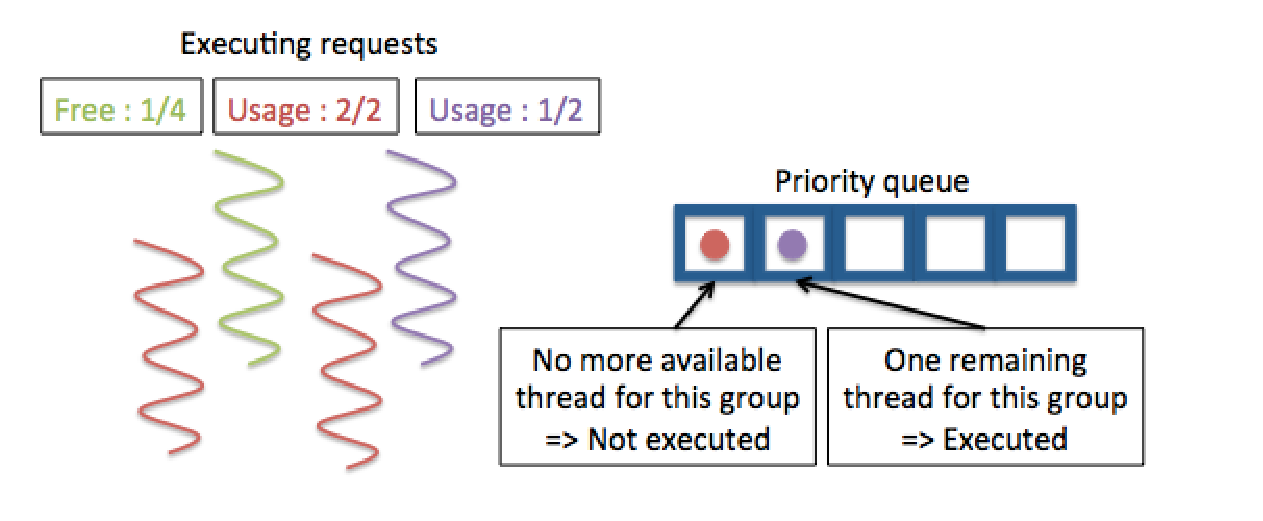
\includegraphics[scale=0.5]{pictures/thread_limit.pdf}
      \end{minipage}
      }
      \caption{An example of request scheduling considering thread limits}
      \label{fig:thread_limit} 
\end{figure}

Nevertheless, considering compatibilities, priorities and thread management, the scheduling of requests within a multiactive object is still deterministic. In the end, priorities can be considered as hints of execution more than strong requirements, but this is needed to balance the execution. No policy can both ensure fairness of requests execution and strong priorities at the same time, because those notions are orthogonal. We attempted to converge towards a scheduling model that is well balanced between the programmer's wishes and a correct execution.


\subsection{Software Architecture}
In this section, we expose the integration of our scheduling mechanisms in the  the global architecture of multiactive objects, as well as we present the main internal structures used to implement them.

A multiactive object intrinsincally embeds an object of type MultiactiveService. The MultiactiveService has two purposes. Firstly, it relies on an AnnotationProcessor that processes annotations to initialize all the structures required by a multiactive object (structures that store compatibilities, priorities and keep tracks of threads). Secondly, the MultiactiveService has a RequestExecutor, that schedules the requests according to compatibilities, priorities and thread class managers. All manager classes rely on the structures previously established when reading annotations. Figure~\ref{fig:uml} displays an UML diagram describing the class composition of a multiactive object, as well as the most important interfaces.

\begin{figure}[!ht]
      \fbox{
      \begin{minipage}[c]{\textwidth}
      \centering
      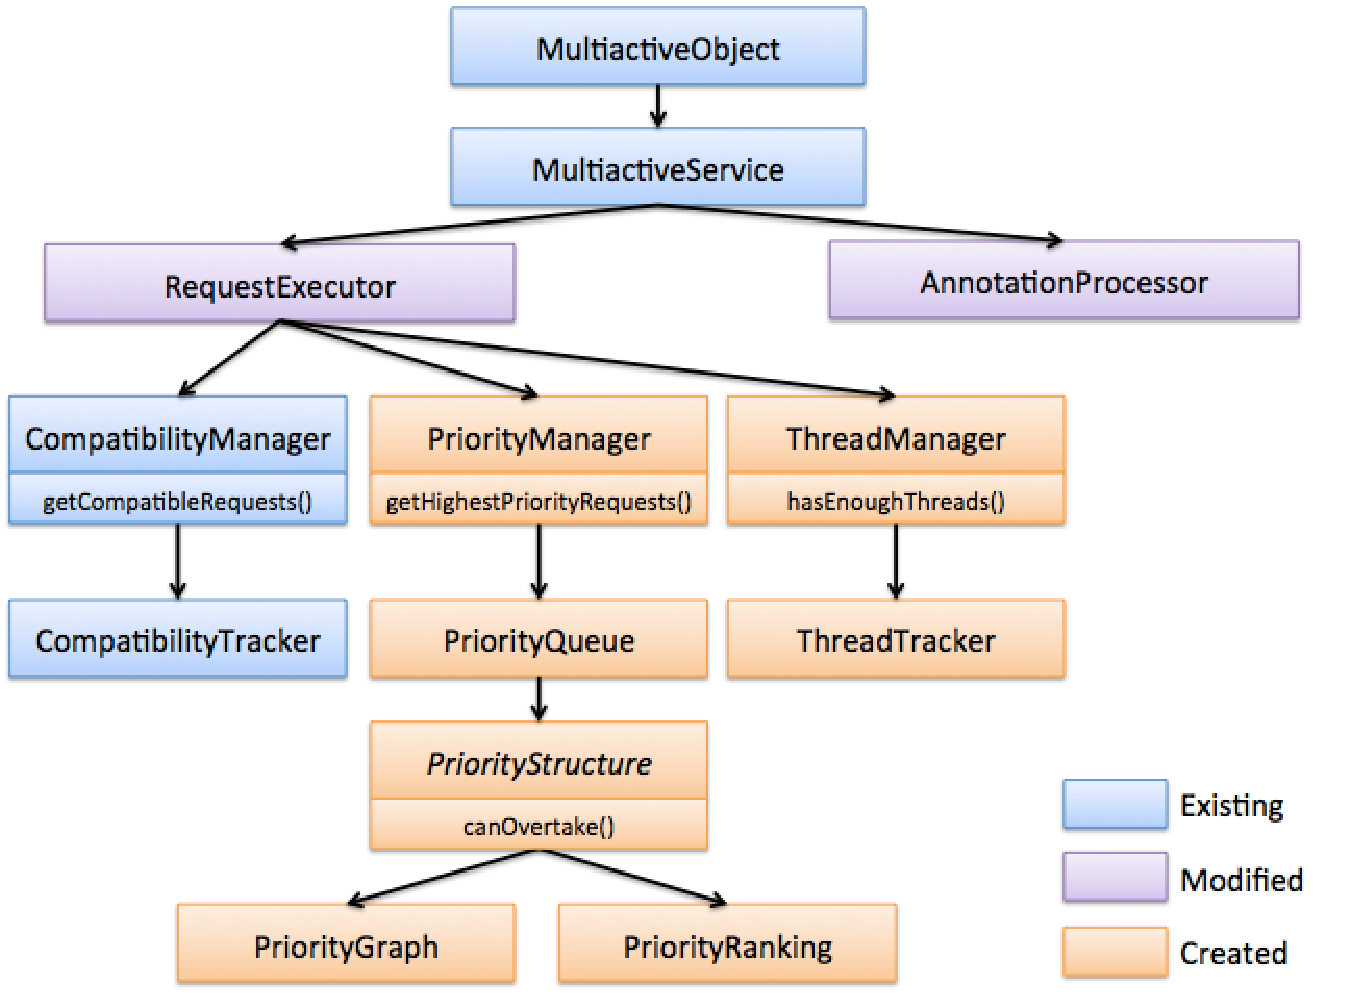
\includegraphics[scale=0.5]{pictures/uml.pdf}
      \end{minipage}
      }
      \caption{Class diagram of multiactive objects with scheduling controls}
      \label{fig:uml} 
\end{figure}

The RequestExecutor has only access to the general interface of compatibility, priority and thread management entities. This general interface enables to retrieve requests of highest priority that are ready to be executed. Each entity manages its own state internally. More precisely, to execute requests, the RequestExecutor first filters incoming requests with the CompatibilityManager. Among compatible requests (request that are ready to be executed safely), a second filter is applied using the PriorityManager, that sends back a list of the highest priority requests. Then, the final decision regarding the execution of a request depends on the ThreadManager, that filters highest priority requests according to the number of threads that are available for them. After applying those three filters sequentially, remaining requests are the ones that should be actually executed. Indeed, each request must satisfy the three steps of compatibilty, priority, and thread availability before being executed. 

The priority mechanism is the most complex. It relies on a customized PriorityQueue (unfortunately, existing implementations could not be used because of specific needs). The PriorityQueue adheres to the producer/consumer design pattern \cite{ref:producerconsumer}. On one hand, a dedicated thread registers compatible requests to the queue. On the other hand, another dedicated thread polls the queue to retrieve highest priority requests. This synchronization is implemented using Java's concurrency mechanisms. When a request is registered to the PriorityQueue, it relies on a PriorityStructure to decide on the insertion position of the request. The actual PriorityStructure used for that can be either our dependency graph (PriorityGraph), or our integer-based priority specification (PriorityRanking). A concrete PriorityStructure should implement the \textbf{canOvertake(request1, request2)} method that says whether a request can be positioned before another one. In the PriorityGraph case, this method goes through the graph to retrieve this information. In the PriorityRanking case, the priority values of the requests are simply retrieved from a tree-based map, which ensures a good efficiency.

This design can easily be adapted to other implementations of active objects, that basically support annotations and their processing using reflexivity. 


\section{Experimental evaluation}\label{sec:experiments}
In this section, we evaluate the performance of the priority mechanism we developed through experiment. 
We show first that our specification is effective: priorities contribute to speed up processing of high priority requests. Secondly, we show that it is efficient: the cost to reorder the queue according to priorities is not high compared to the time needed to serve a request.

\subsection{Environment}
All experiments were run on a single machine. Indeed, we evaluate priorities in a parallel execution context. But here, we want to evaluate request parallelism, which occurs within a multiactive object. Thus, even though the context of multiactive objects is distributed, we only need to run experiments on one machine, because request parallelism using priorities occurs only within one multiactive object, which lies on one machine. Our mechanism only contribute to the efficiency of local parallelism, not to the efficiency of distributed execution.

The machine has 

When the priority specification that is used is not mentioned, it means that we are using our graph-based specification.
At the beginning of each experiment, we send one big request per available thread to ensure that all the requests we evaluate are inserted in the queue before we start executing them.

In all experiment, all the considered groups are compatible, otherwise, they would never be in the ready queue at the same time, and we could never apply priorities on the requests belonging to them.

machine config,
taille des queues,
duree des methodes,
compatibility settings,
graph settings

\subsection{Speed up of high priority requests}
In this experiment, we define only two groups: A and B. Each group has only one request that is assigned to them. We send in total 1000 requests to a multiactive object that we have previously defined: alternatively a request of group A and a request of group B. So each group sends 500 requests. We run two executions. In the first execution we do not declare any priority relation between group A and group B. In the second execution, we declare a priority dependency from group A to group B. We evaluate the execution time dynamic of requests of group A and requests of group B. The execution time is composed by the time to insert the request in the ready queue + the waiting time in the ready queue + the service time of the request. To perform this evaluation, we average execution times of requests by batch of 50 consecutive requests of the same group. Figure A depict the results of both executions:

\TODO{figure}

When not using priorities, the execution time of requests increases equally for both groups as the ready queue increases. As expected, when using priorities, the execution time of requests of group A is divided by two and the execution time of requests of group B is doubled. As a comparative evaluation, with no priorities, after 30ms 200 requests of group A have been executed. With priorities, at the same point in time, more than 400 requests of group A have been executed. It means that after only 30ms of request processing, we have already a speed up of 2 for high priority requests. This shows that our priority specification is effective: it successfully speeds up the execution of high priority requests. 

augmenter throughput of high priority requests
montrer qu'on effectue plus de high priority requests en un temps donne : pour executer ce lot de requetes il me faut Xs et avec priorite il me faut seulement Ys.
dire : for only X\% of overhead we are able to speedup the execution of the most important requests of X\%. 


\subsection{Overhead of the different priority specifications}
In this section, we perform two experiments that evaluate the overhead of the priority specifications. We define the overhead of a given priority mechanism as the time needed to insert an incoming request in the queue, according to its priority. When no priority mechanism exists, such overhead is quasi null: the request is just put at the end of the queue, which is a constant operation. However, with our priority mechanisms, we have seen that we potentially have to look through the whole ready queue to find the right position of an incoming request. As a consequence, this operation is dependent on the number of requests that already are in the queue. In addition, the structures used to store priorities and to decide on overtakability of requests are also a factor of complexity of the insertion process. In our case, we have two priority specifications that rely on two different structures: a linear structure and a graph structure. We evaluate both of them to see if the overhead of our graph-based specification is not too high. 

\subsubsection{Alternative high and low priority requests}
For this experiment, we define five groups and their priority. We declare the priorities on one hand using the integer-based specification and on the other hand using the graph-based priority specification. The exact priorities applied are displayed on figure X.

\TODO{figure}



We send 1000 requests to a multiactive object previously defined. Our goal is to send alternatively a request of highest priority and a request of lowest priority, so that 500 requests for each of the two groups. We perform two runs: one using the integer-based specification and one using the graph-based specification. Figure X shows the results of both priority specifications for both kind of requests:

\TODO{figure}




\subsubsection{Sequential requests belonging to a non-naive graph}
To illustrate a more realistic case, we create in this usecase nine groups, each of them having a single belonging request. The priority dependencies are expanded in Figure X:

\TODO{figure}

To evaluate the cost of the graph-based specification, we attempt to translate this dependency graph into integer-based priorities. As for this dependency graph it is not possible to have the exact same semantics with integer, we define priorities the closest they can be to the dependency graph. The resulting translation is displayed on Figure X:

\TODO{figure}

We sequentially send a request of each group in a previously defined order. The sequence of requests are sent in the following order:
\begin{enumerate}
\item g7
\item g1
\end{enumerate}
This sequence of requests allows us to have deterministic results while experimenting all parts of the graph. In total, 500 requests are sent per group, which makes 4500 requests sent to the multiactive object in total.

The results are displayed on Figure X.

\TODO{figure}
As the previous usecase, the overhead of the graph-based priority specification is slightly higher than the overhead of the integer-based specification. But in this usecase, the difference between the two specifications is bigger: the overhead is here twice higher, whereas it was only 1.5 higher in the previous usecase.
This is explained by the fact that the graph is more complex in the later usecase. So we can guess that the more complex the graph is (the more nodes and dependencies it has), the bigger is the overhead of the graph-based priority specification.
But in practice, the graph has few chances to be highly complex because it would require the multiactive object to have a lot of methods defined, and in a well-designed object-oriented application, objects must have a concise and precise purpose, which is antagonistic with having a lot of methods. Also, receiving more than 4000 requests at the same time is not an usual situation. In this extreme case still, our graph-based priority specification represents only twice the overhead introduced by the integer-based priority specification. Considering the ease of usage that the graph-based priority specification offers, it is a small cost. On the other hand, this overhead represents only X\% of the service time of the request, which is negligible. To conclude, the experiment showed that the graph-based priority specification is adapted to a practical usage, because it is efficient, in addition to be easy to use and very expressive. 


\chapter{Conclusion and Future Work} 
\section{Conclusion}
In this report, we presented several mechanisms to allow the programmer to control more finely request scheduling of multiactive objects. All mechanisms offer new annotations that we have developed. Annotations can be seen as meta programming facilities, and using them is much more simpler than coding the intended behavior directly in the business model. This way, scheduling hints are given in a declarative fashion, and then the corresponding code is automatically executed. Related works on high-level scheduling did not provide such an abstract specification, or were fairly complex to use. In most of the cases, they imply to write business code and ask for a large knowledge of the programmer. In our work, we succeeded in providing a high level language to specify scheduling hints.

The first scheduling mechanism that we have introduced gives the possibility to assign different priorities to group of requests, in order to prioritize the execution of requests. For that, we developed two priority specifications. The first priority specification we developed is a classical approach when dealing with priorities: it consists in ordering requests according to integer order. The programmer uses this order to assign priorities to group of requests. The second priority specification we have developed is more elaborated than the first one. It relies on a dependency graph: when a group has a higher priority than another, a dependence is created between them. This specification is simpler to use, and more expressive, but requires more processing resources. We developed both specifications in order to evaluate them in practice: we want to select the one that is well balanced between ease of programming and efficiency.

We have also developed a scheduling mechanism that can be used to control thread allocation in a multiactive object. We have seen that this particular scheduling mechanism was needed to prevent starvation of requests in some cases. The principle of this mechanism is simple: it consists in defining an upper and lower bound on the number of threads that can be occupied by requests of a given group at a time. As it is mainly based on the programmer's consciousness, we chose to override specifications that were not conform to our vision of safety of execution.

Finally, we ran experiments of the priority mechanism. Firstly, we showed that the priority mechanism increased significantly the processing of high priority requests. This was a necessary experimentation, first to show that the result was the one expected, and second because we modified the priority enforcement by introducing our thread allocation mechanism. In particular, despite the fact that we control allocation of threads over priorities, we still get the expected behavior. The second experimentation showed that our priority specification based on a dependency graph introduced a bearable overhead. Indeed, the insertion of a request in our priority queue using the graph represents only a minor part of the sojourn time of a request. To summarize, experiments validated the use of graph-based priorities, because this specification is easier to use, offers a larger expressiveness, and keeps a low overhead compared to classical approaches of priorities. 


In conclusion, we enlarged the multiactive object model so that it can benefit from low level concurrency customization and also from high level programming and execution safety. Schematically, the multiactive object were located in between the strict, safe model of active objects, and the very permissive, error prone low level concurrency mechanisms. In this work, we contributed to broaden the scope of multiactive objects, while trying to keep a safe control over multiactive object executions. Therefore, up to now, the multiactive object model is the most complete model to provide both distributed \emph{and} concurrent mechanisms in the same abstraction, while remaining simple and safe.



\section{Future work}
The multiactive object model is still a recent design that needs further work to be finalized. The very next goal is to experiment our scheduling mechanisms in a real case. Indeed, the experiments presented in this work were built to test our scheduling mechanisms at their limits, but we would like now evaluate their impact in a real context. The EventCloud platform \cite{ref:eventcloud} is currently developed in the team using multiactive objects. Its goal is to handle notification deliveries in a peer-to-peer manner. We would like to develop a particular usecase using this platform to demonstrate the utility of our scheduling mechanisms. 

Also, we would like to explore other ways to manage the threads than the ones we gave. Indeed, our priority mechanism seems to be finalized but our thread management mechanism has not been developed enough to be sure of its optimality, due to lack of time. Although efficient, our thread management mechanism might not be the best to avoid starvation, nor to ensure a maximum utilization. We will probably have to inspire our work from operating system mechanisms to handle those problems.

In a very long term, the multiactive objects will be the basis of  accomplishment of the PhD that I will begin next autumn and that is supervised by Ludovic Henrio \cite{ref:these}. The main goal of this PhD is to design a fault tolerant programming model adapted to (globally) distributed and (locally) concurrent applications. We will use multiactive objects as concrete implementation of such models. Briefly, the problematic is that fault tolerant protocols for distributed systems have all been designed following the same assumption: messages sent from one entity to another should follow a first in first out policy. But as multiactive objects introduce other complex scheduling policies, such protocols cannot be used any more to ensure a correct fault tolerance of multiactive objects. Although ad hoc mechanisms exist to handle other policies and still get a good fault tolerant mechanism, no general model is provided to handle fault tolerance in a generic manner. To reach this objective, we will use the scheduling tools developed in this work. First, our priority specification will be essential to process in priority requests that are devoted to fault tolerance. Second, we will use our analysis of request scheduling of multiactive objects to converge towards a general model for adaptive fault tolerance of distributed and concurrent systems.


\bibliographystyle{plain}
\bibliography{biblio}

\end{document}

Note : consider building the graph of transitive closure to determine faster the reachability (experimentations)

Note : notion de hard priorite

Compilation time verified annotation (example: check that groups exist)

annexe : JAVA 8 annotations vs JAVA 7 -> much lighter


INDEX
active object
multiactive object
Future
request
starvation
priority inversion

